\begin{donnees}
    \begin{itemize}
        \item $m=\qty{0,2}{\kg}$~; les frottements sont négligeables.
    \end{itemize}
\end{donnees}
On écarte le solide $\mathrm{(S)}$ (Fig.~\ref{fig:solide_ressort}) de sa
position d'équilibre d'une distance $X_{m}=\qty{2}{\cm}$ et on le libère sans
vitesse initiale à l'instant $t_{0}=0$.

On choisit l'état où le ressort n'est pas déformé comme référence de l'énergie
potentielle élastique $E_{pe}$ et le plan horizontal contenant
G comme état de référence de l'énergie potentielle de pesanteur
$E_{pp}$.

\begin{minipage}{0.59\linewidth}
    La Fig.~\ref{fig:2bac_svt_national_2017_rattrapage_phys_ex3_4} représente
    les variations de l'énergie potentielle élastique $E_{pe}$ et de l'énergie
    cinétique $E_{c}$ en fonction du temps pour l'oscillateur étudié.
    \begin{enumerate}
        \item Montrer, que la courbe~(2) correspond à l'énergie cinétique
              $E_{c}$ du système oscillant.
        \item Déterminer graphiquement, la valeur de l'énergie potentielle
              élastique maximale $E_{pe,\max}$.
        \item En déduire la valeur de la raideur $K$.
        \item Déterminer la valeur de la vitesse $v_{G}$ du centre d'inertie $G$
              lorsque $E_{c}=E_{pe}$.
    \end{enumerate}
\end{minipage}
\begin{minipage}{0.40\linewidth}
\begin{figure}[H]
    \centering
    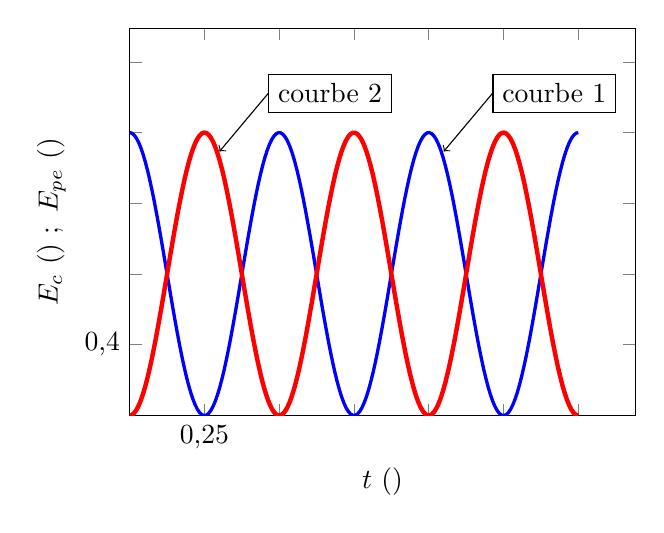
\begin{tikzpicture}
        \def\Xm{0.02}
        \def\T{1}
        \def\K{8}
        \pgfmathpi\let\pi=\pgfmathresult
        \begin{axis}[
                xmin=0,xmax=1.69,
                ymin=0,ymax=2.19,
                width=8cm,height=6.5cm,
                trig format plots=rad,
                xtick distance=0.25, ytick distance=0.4,
                xticklabels={,,{0,25}}, yticklabels={,,{0,4}},
                xlabel=$t~(\unit{\second})$,
                ylabel=$E_{c}~(\unit{\mJ})~;~E_{pe}~(\unit{\mJ})$,
                minor tick num=0,
            ]
            \addplot[domain=0:1.5,samples=200,very thick,blue]
                {0.5*\K*\Xm*\Xm*cos(2*pi/\T*x)*cos(2*pi/\T*x)*1e3}
                coordinate[pos=0.68] (c1);
            \addplot[domain=0:1.5,samples=200,ultra thick,red]
                {0.5*\K*\Xm*\Xm*sin(2*pi/\T*x)*sin(2*pi/\T*x)*1e3}
                coordinate[pos=0.18] (c2);
        \end{axis}
        \draw[<-,shorten <=1pt] (c1) -- ++(50:1) node[right,draw] {courbe~1};
        \draw[<-,shorten <=1pt] (c2) -- ++(50:1) node[right,draw] {courbe~2};
    \end{tikzpicture}
    \caption{}
    \label{fig:2bac_svt_national_2017_rattrapage_phys_ex3_4}
\end{figure}
\end{minipage}

